\begin{section}{Parameterizing \cus-\mof force fields with \lmoeda}
\label{sec:lmoeda-theory}

Based on the results for \mgmof, it is clear that, at least for \cus-\mofs, a
new methodology is required which simultaneously keeps the important advantages of the
old development strategy (especially the component-by-component based parameterization,
which is essential for generating transferable force fields) while overcoming
the limitations of \sapt itself. Put differently, for \cus-\mofs we should
seek a new electronic structure theory benchmark and associated \eda 
with the following qualities:
%
\begin{enumerate}
\item High accuracy with respect to to \ccsdtf benchmark energies
\item Physically-meaningful energy decomposition into (at least)
electrostatics, exchange, induction, and dispersion
\item Quantitative correspondence
between the energy decompositions of \sapt and the new method for systems
where total energies from \sapt, \ccsdtf, and the new method agree
\end{enumerate}
%
Assuming these three qualites are met, we expect to be able to generate force
fields for \cus-\mofs that are both highly accurate and maximally-compatible
with previous force fields developed for coordinatively-saturated \mof
systems. 

A substantial number of \glspl{eda} exist in the literature,
and the interested reader is referred to \citen{Pastorczak2017} for a
review and comparison of various popular methods. Aside from \sapt, which is a
perturbative method, most \edas are `variational', meaning that the
various energy components are calculated in stages from a series of constrained
relaxations of the monomer wavefunctions into the optimized
dimer wavefunction. For this reason, all variational \edas
are guaranteed to have total energies that match the result from a supermolecular
interaction energy calculation. Furthermore, these \edas are often implemented
for wavefunction and \dft methods, thus allowing for significant
flexibility (compared to the \sapt \eda) in terms of finding an \eda whose
total energy closely matches \ccsdtf. Indeed, and 
as shown in
\cref{fig:lmoeda-sapt_breakdown}, \pbeod
shows excellent agreement with \ccsdtf for a \mgmof cluster model, 
and so any \dft-compatible \eda should meet our first criteria from above.

Although all variational \edas yield the same
total interaction energy for a given level of theory, many \edas can differ substantially in terms of how
this total energy is decomposed into chemically-meaningful components. At the
time this research was completed, only a handful of variational \edas distinguished each
electrostatics, exchange, induction, and dispersion. (Notably, the recent
second-generation ALMO-EDA\cite{Horn2016b} now
separates their `frozen' energy term into electrostatic, exchange, and
dispersion components, and thus might be worth future investigation.) Of the
popular \eda methods available in 2014, we found that
\lmoeda,\cite{Su2009,Chen2010}
GKS-EDA,\cite{Su2014} and PIEDA\cite{Fedorov2006} decompose the total
interaction in a manner philosophically similar to \sapt, and include each
electrostatic, exchange, induction, and dispersion terms. These three methods
thus meet our second criteria for
an optimal energy decomposition scheme for \cus-\mofs, and complete formalisms and
details for the methods can be found in \citens{Su2009,Chen2010,Su2014,Fedorov2006}.

As for the last criterion, that of maximum correspondence between \sapt and a
variational \eda, we have performed component-by-component analyses
to compare \sapt to both \lmoeda and GKS-EDA. PIEDA is known to
overestimate the relative magnitude of the polarization energy, compared to
\sapt, and thus was not considered in detail.\cite{Pastorczak2017} As for
\lmoeda and GKS-EDA (both of which are based on very similar theories, and
tend to yield similar energy decompositions), we have in
general found semi-quantitative to quantitative agreement with the \sapt
energy decomposition, particularly for the electrostatic and exchange
energies. Comparisons between \lmoeda and \sapt are shown for the \co dimer
(\cref{fig:lmoeda-co2_co2}) and for \co interacting with a model \mgmof
compound (\cref{fig:lmoeda-co2_mgmof}). GKS-EDA results are not shown, as
the \lmoeda and GKS-EDA results tend to be very similar, with the GKS-EDA
results in slightly worse agreement with \sapt. For this reason, and because
\lmoeda does the best job of meeting our three criteria above, we choose in
this work to use \lmoeda as our new benchmark \eda for fitting \cus-\mof force
fields.


    %%%%%%%%%%%% CO2 Dimer PES %%%%%%%%%%%%%%%%
    \begin{figure}
    \centering
    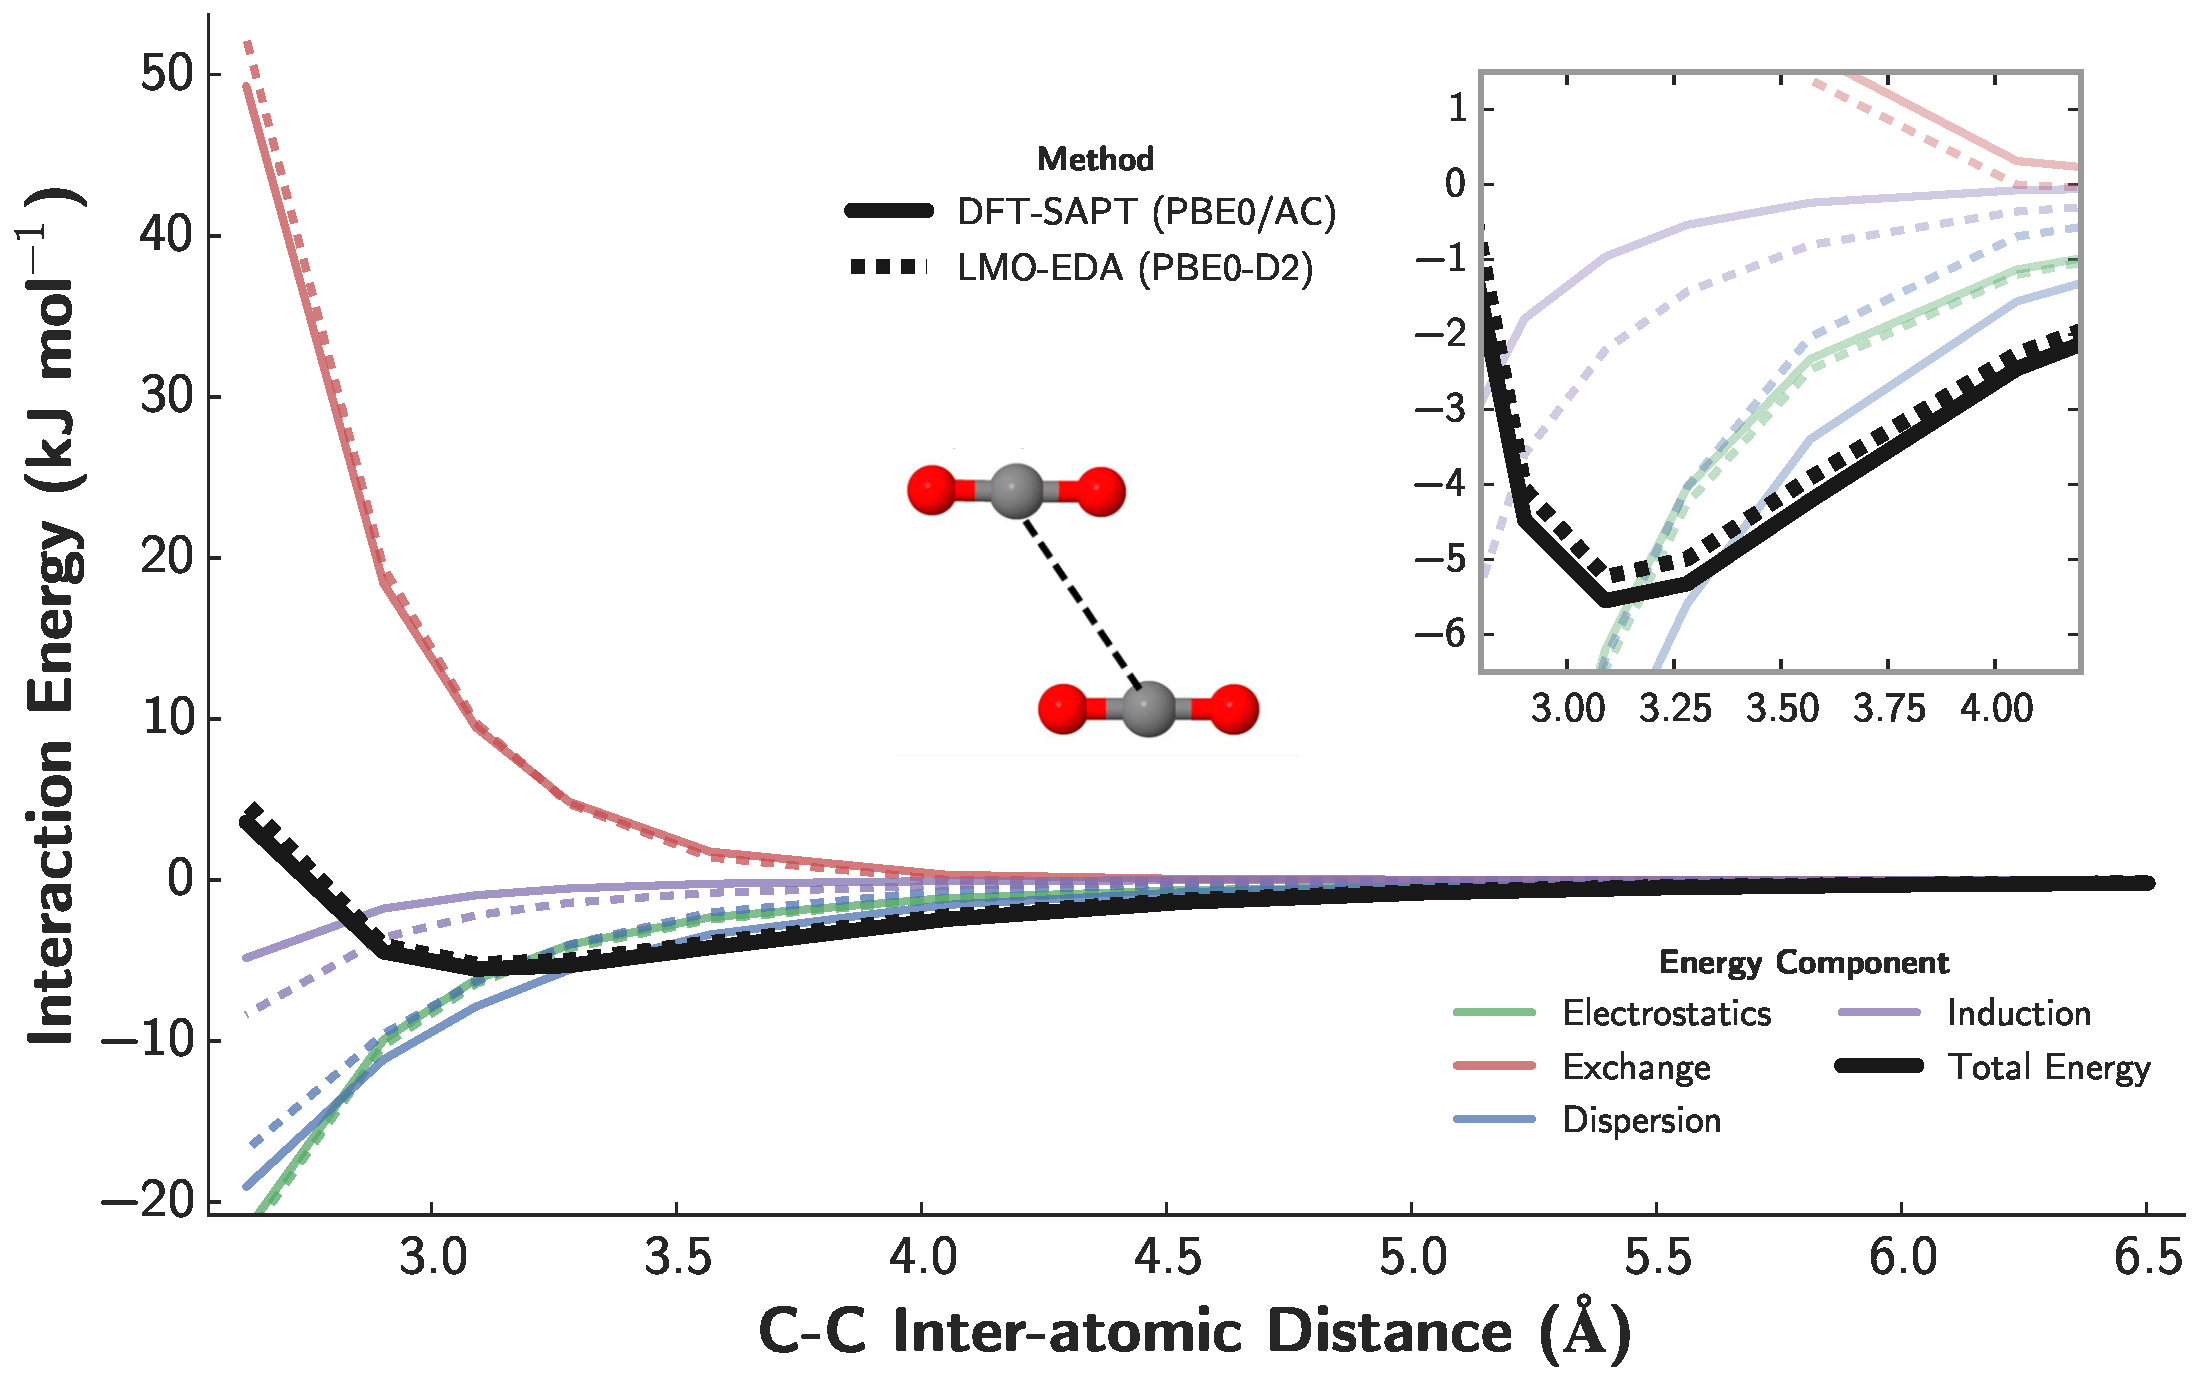
\includegraphics[width=1.0\textwidth]{lmoeda/co2_co2_pes.pdf}
    \caption[\lmoeda vs. \sapt \pes for the \co dimer]
{\pes and associated energy decomposition for the slipped parallel geometry of
the \co dimer as a function of
the \ch{C-C} interatomic distance. The \pes has been
computed by both \dftsapt(PBE0) (solid lines) and \lmoeda-\pbeod (dashed
lines), and each electrostatics (green), exchange (red), dispersion (blue),
induction (purple), and total energy (black) components are displayed.
Note that, for the \dftsapt energies, the \dhf contribution has been
incorporated into the \induction energy.
            }
    \label{fig:lmoeda-co2_co2}
    \end{figure}
    %%%%%%%%%%%% CO2 Dimer PES %%%%%%%%%%%%%%%%

    %%%%%%%%%%%% CO2 Mg-MOF-74 PES %%%%%%%%%%%%
    \begin{figure}
    \centering
    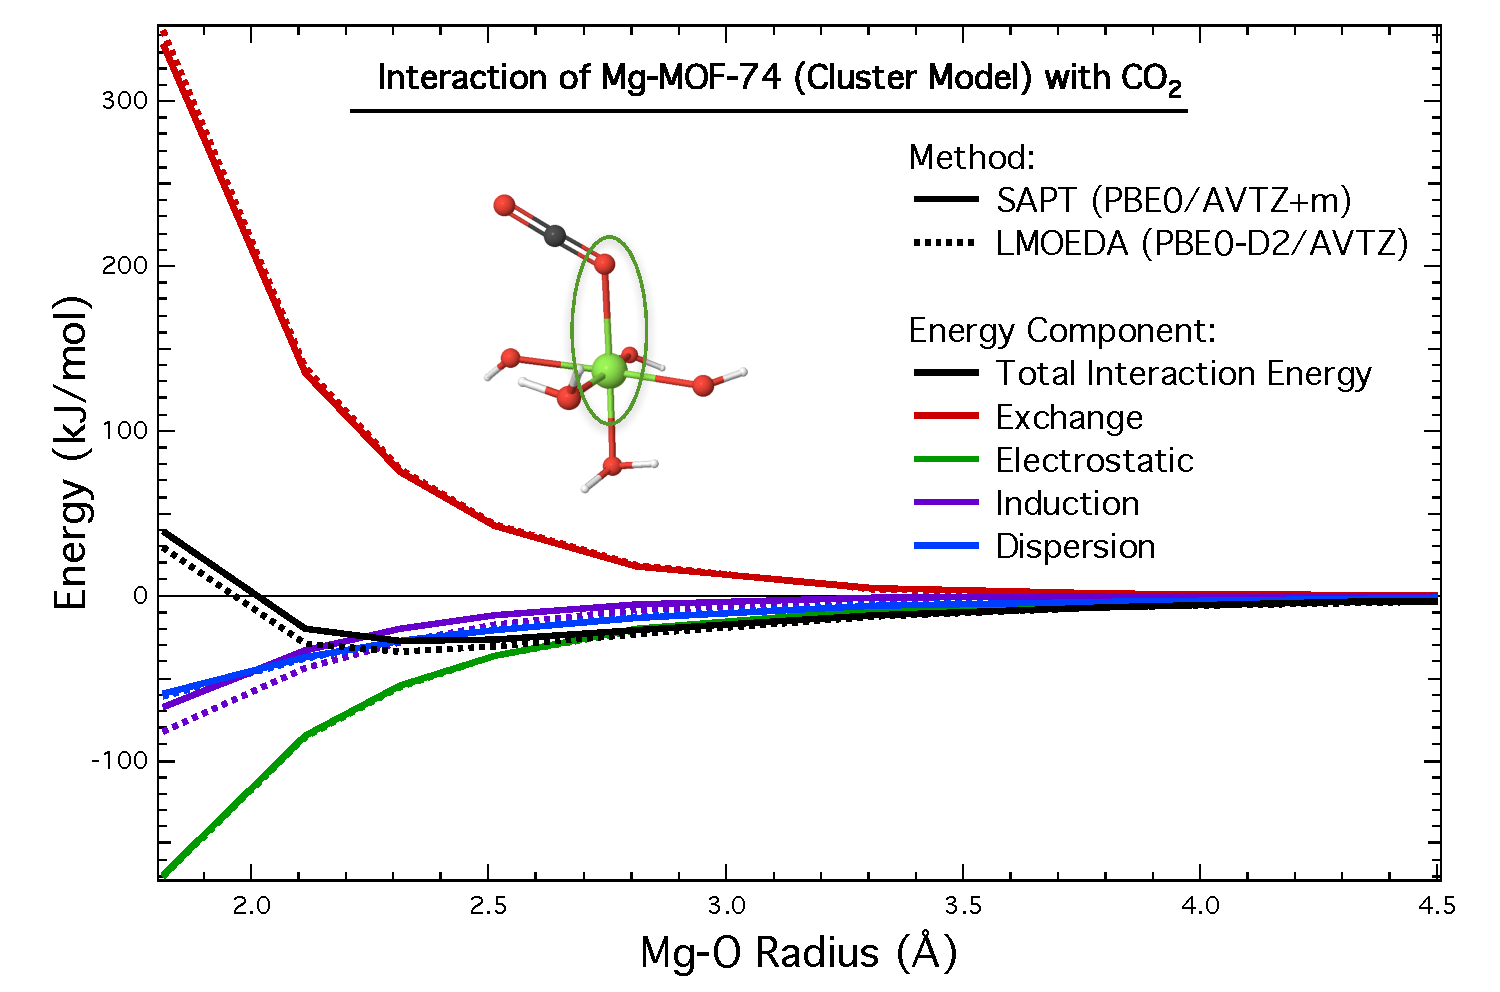
\includegraphics[width=1.0\textwidth]{lmoeda/co2_mgmof_pes.pdf}
    \caption[\lmoeda vs. \sapt \pes for the \co/\mgmof dimer ]
{\pes and associated energy decomposition for a \co + \ch{MgO5} cluster, 
as a function of the highlighted \ch{Mg-O} interatomic distance. 
The \pes has been
computed by both \dftsapt(PBE0) (solid lines) and \lmoeda-\pbeod (dashed
lines), and colors and labels for the energy decomposition are as in
\cref{fig:lmoeda-co2_co2}. 
            }
    \label{fig:lmoeda-co2_mgmof}
    \end{figure}
    %%%%%%%%%%%% CO2 Mg-MOF-74 PES %%%%%%%%%%%%

In addition to describing the advantages of the \lmoeda method, it is worthwhile to overview
some of its relevant shortcomings and limitations. 
As with most variational \eda methods,\cite{Pastorczak2017} and especially for
\dft-based methods, it becomes difficult to precisely assign and separate out the true
`dispersion' energy for a system. This limitation is also true of \lmoeda,
where the dispersion energy is defined as the difference in correlation energy
between the monomer and dimer wavefunctions. (For density functionals employing
Grimme's --D dispersion correction, this correction is also added to the
\lmoeda dispersion energy.) For functionals that have a well-defined and
theoretically-grounded distinction between the exchange and correlation
functionals, the \lmoeda energies tend to agree well with \sapt, and we have
found good agreement (for instance) between \sapt and \lmoeda-\pbeod. With other
functionals, such as with our tests using the M06 functional, there is no
separation between the exchange and correlation functionals, and \lmoeda gives
unphysical values for both the exchange and dispersion energies in this case.
(Notably, GKS-EDA attempts to rectify this issue by changing the \lmoeda formalism for
dispersion. While this leads to qualitative agreement between \sapt and
GKS-EDA for a wider variety of functionals, the quantitative agreement for the
\pbeod functional is somewhat worsened for the systems studied herein, and we
instead use \lmoeda-\pbeod for all results in this work.)

A second, and purely practical, limitation of \lmoeda is its memory-intensive
implementation in GAMESS. As will be discussed in detail later,
calculations on a large (43 heavy atom) cluster model of \mgmof were
infeasible for us (using the Phoenix cluster in 2014) in all but the smallest VDZ
basis set, and calculations on an identical cluster model of \comof could not
be completed at all. For this reason, the \lmoeda method is practically
restricted to studies of smaller systems and/or basis sets.


\end{section}
